%% VLA-Finance Weekly Report Slides
%% Overleaf: New Project -> Blank -> paste into main.tex -> Recompile (PDFLaTeX)
\documentclass[aspectratio=169,11pt]{beamer}

% ── Theme ──────────────────────────────────────────────────────────
\usetheme{Madrid}
\usecolortheme{whale}
\setbeamertemplate{navigation symbols}{}
\setbeamertemplate{footline}[frame number]

% ── Packages ───────────────────────────────────────────────────────
\usepackage{booktabs}
\usepackage{multirow}
\usepackage[table]{xcolor}
\usepackage{tikz}
\usetikzlibrary{arrows.meta, positioning, shapes.geometric}
\usepackage{array}
\usepackage{amsmath}

% ── Colors ─────────────────────────────────────────────────────────
\definecolor{trainblue}{RGB}{52,120,190}
\definecolor{valgreen}{RGB}{60,160,60}
\definecolor{testred}{RGB}{200,60,60}
\definecolor{bestcol}{RGB}{0,80,200}
\definecolor{rowgray}{gray}{0.93}

\newcommand{\best}[1]{\textcolor{bestcol}{\textbf{#1}}}

% ── Title ──────────────────────────────────────────────────────────
\title[VLA-Finance]{VLA Framework for Bitcoin Price Prediction}
\subtitle{Weekly Experiment Report}
\author{}
\date{\today}

% ═══════════════════════════════════════════════════════════════════
\begin{document}
% ═══════════════════════════════════════════════════════════════════

\begin{frame}
  \titlepage
\end{frame}

\begin{frame}{Outline}
  \tableofcontents
\end{frame}

% ───────────────────────────────────────────────────────────────────
\section{1. Previous Experiment Recap}
% ───────────────────────────────────────────────────────────────────

\begin{frame}{Previous Experiments --- Design Space Explored}
  \begin{columns}
    \begin{column}{0.48\textwidth}
      \begin{block}{Action Representation}
        \begin{itemize}
          \item \textbf{log-ratio}: $\log(p_t / p_{\text{last}})$ --- all steps relative to last close
          \item \textbf{delta}: $\log(p_t / p_{t-1})$ --- each step relative to previous candle
        \end{itemize}
      \end{block}
      \begin{block}{Input Modality}
        \begin{itemize}
          \item Image + Text (chart image included)
          \item \textbf{Text-only} (image removed)
        \end{itemize}
      \end{block}
    \end{column}
    \begin{column}{0.48\textwidth}
      \begin{block}{Action Head}
        \begin{itemize}
          \item MLP (QwenOFT)
          \item DiT-B / Flow Matching (GR00T)
        \end{itemize}
      \end{block}
      \begin{block}{Candle Granularity}
        \begin{itemize}
          \item 15-min, 30-min, \textbf{1-hour}
        \end{itemize}
      \end{block}
    \end{column}
  \end{columns}

  \vspace{0.5em}
  \begin{alertblock}{Finding}
    Among all combinations, \textbf{v9\_delta} (QwenOFT + MLP + delta target + text-only)
    performed best --- especially at prediction horizon \textbf{k=6}
  \end{alertblock}
\end{frame}

\begin{frame}{Previous Experiments --- v9\_delta vs.\ Kronos (Single Test Period)}
  \begin{table}
    \centering
    \renewcommand{\arraystretch}{1.4}
    \begin{tabular}{lcccc}
      \toprule
      \textbf{Model} & \textbf{DA} $\uparrow$ & \textbf{Long\_ns} & \textbf{AER} $\uparrow$ & \textbf{MDD} $\uparrow$ \\
      \midrule
      \rowcolor{rowgray}
      Kronos (baseline) & 0.515 & 0.300 & $-$0.116 & $-$0.104 \\
      \textbf{v9\_delta}    & \best{0.544} & 0.375 & \best{$+$0.058} & \best{$-$0.046} \\
      \bottomrule
    \end{tabular}
    \par\vspace{0.3em}\centering\footnotesize Prediction horizon $k=6$ / Slippage 0.1\%
  \end{table}

  \vspace{0.3em}
  \begin{block}{Interpretation}
    \begin{itemize}
      \item DA 54.4\% vs.\ Kronos 51.5\% --- better directional accuracy
      \item AER \textbf{+5.8\%} --- positive excess return over BTC buy-and-hold
      \item However, this result is from a \textbf{single test period} (2026-03) --- reliability limited
      \item[$\Rightarrow$] Need a more rigorous evaluation protocol
    \end{itemize}
  \end{block}
\end{frame}

% ───────────────────────────────────────────────────────────────────
\section{2. This Week's Experiment Setup}
% ───────────────────────────────────────────────────────────────────

\begin{frame}{2-1. Walk-Forward 6-Fold Cross-Validation}
  \begin{columns}
    \begin{column}{0.42\textwidth}
      \begin{block}{Problem with Previous Setup}
        \begin{itemize}
          \item Single train/val/test split
          \item Results biased toward one market period
          \item Cannot capture regime changes (bull/bear)
        \end{itemize}
      \end{block}
      \begin{exampleblock}{New Evaluation Protocol}
        \begin{itemize}
          \item \textbf{Walk-forward 6-fold} (2020--2025)
          \item Each year evaluated independently
          \item Checkpoint selection: maximize val $\text{DA}_{k=6}$
        \end{itemize}
      \end{exampleblock}
    \end{column}
    \begin{column}{0.54\textwidth}
      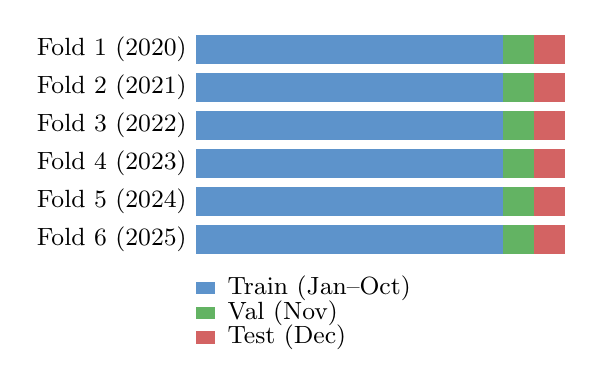
\begin{tikzpicture}[scale=0.78, every node/.style={font=\small}]
        \foreach \fold/\yr in {1/2020,2/2021,3/2022,4/2023,5/2024,6/2025}{
          \pgfmathsetmacro{\y}{(6-\fold)*0.62}
          \fill[trainblue!80] (0,\y) rectangle (5.0,\y+0.48);
          \fill[valgreen!80]  (5.0,\y) rectangle (5.5,\y+0.48);
          \fill[testred!80]   (5.5,\y) rectangle (6.0,\y+0.48);
          \node[left] at (0,\y+0.24) {Fold \fold\ (\yr)};
        }
        % Legend — 3 lines
        \fill[trainblue!80] (0,-0.65) rectangle (0.3,-0.45);
        \node[right, font=\small] at (0.35,-0.55) {Train (Jan--Oct)};
        \fill[valgreen!80]  (0,-1.05) rectangle (0.3,-0.85);
        \node[right, font=\small] at (0.35,-0.95) {Val (Nov)};
        \fill[testred!80]   (0,-1.45) rectangle (0.3,-1.25);
        \node[right, font=\small] at (0.35,-1.35) {Test (Dec)};
      \end{tikzpicture}
    \end{column}
  \end{columns}
\end{frame}

\begin{frame}{2-2. GR00T Architecture --- MLP vs.\ DiT-B}
  \begin{columns}
    \begin{column}{0.48\textwidth}
      \begin{block}{Previous: QwenOFT + MLP (v9\_delta)}
        \begin{itemize}
          \item Qwen3-VL-4B $\rightarrow$ MLP head (regression)
          \item Single forward pass, direct 12-step prediction
          \item Simple but limited expressiveness
        \end{itemize}
      \end{block}
    \end{column}
    \begin{column}{0.48\textwidth}
      \begin{exampleblock}{New: QwenGR00T + DiT-B (v12--v14)}
        \begin{itemize}
          \item Qwen3-VL-4B $\rightarrow$ \textbf{DiT-B} Diffusion Head
          \item \textbf{Flow Matching} (4 inference steps)
          \item \textbf{DCT Loss} ($w{=}0.1$)\\frequency domain supervision
          \item \textbf{ETH Auxiliary Loss} ($w{=}0.5$)\\co-predict Ethereum price
          \item Same delta target representation
        \end{itemize}
      \end{exampleblock}
    \end{column}
  \end{columns}
\end{frame}

\begin{frame}{2-2. GR00T Architecture --- Model Diagram}
  \centering
  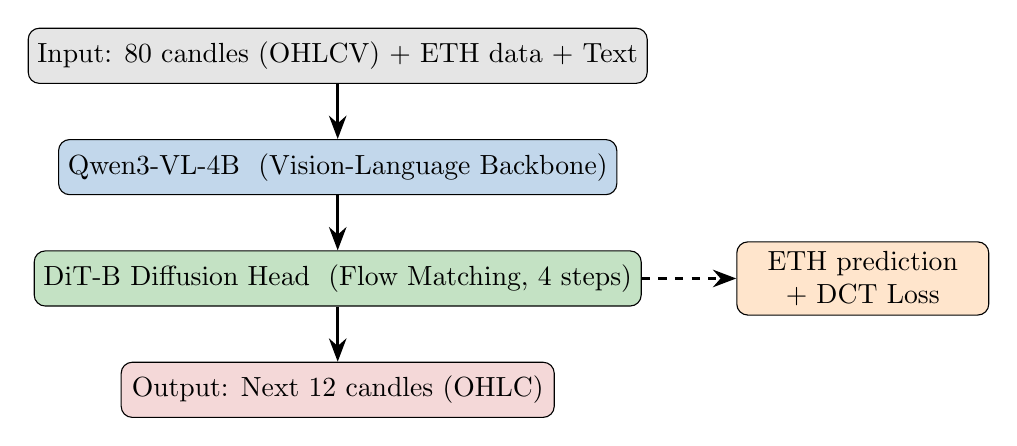
\begin{tikzpicture}[
    node distance=0.7cm,
    box/.style={draw, rounded corners, minimum width=5.5cm,
                minimum height=0.7cm, align=center, font=\normalsize},
    arr/.style={-{Stealth}, thick, line width=1.2pt}
  ]
    \node[box, fill=gray!20] (input)
      {Input: 80 candles (OHLCV) + ETH data + Text};
    \node[box, fill=trainblue!30, below=of input] (vlm)
      {Qwen3-VL-4B \ (Vision-Language Backbone)};
    \node[box, fill=valgreen!30, below=of vlm] (dit)
      {DiT-B Diffusion Head \ (Flow Matching, 4 steps)};
    \node[box, fill=testred!20, below=of dit] (out)
      {Output: Next 12 candles (OHLC)};
    \node[box, fill=orange!20, right=1.2cm of dit, minimum width=3.2cm] (aux)
      {ETH prediction\\+ DCT Loss};
    \draw[arr] (input) -- (vlm);
    \draw[arr] (vlm)   -- (dit);
    \draw[arr] (dit)   -- (out);
    \draw[arr, dashed] (dit) -- (aux);
  \end{tikzpicture}
\end{frame}

\begin{frame}{Model Summary}
  \begin{table}
    \centering
    \renewcommand{\arraystretch}{1.4}
    \begin{tabular}{llcccc}
      \toprule
      \textbf{Model} & \textbf{Action Head} & \textbf{Candle} & \textbf{Target} & \textbf{DCT} & \textbf{ETH} \\
      \midrule
      \rowcolor{rowgray}
      Kronos      & LM (direct gen.)  & 1h           & absolute  & ---        & --- \\
      v9\_delta   & MLP               & 1h           & delta     & \checkmark & \checkmark \\
      \rowcolor{rowgray}
      v12 GR00T   & DiT-B (flow)      & \textbf{15m} & delta     & \checkmark & \checkmark \\
      v13 GR00T   & DiT-B (flow)      & \textbf{30m} & delta     & \checkmark & \checkmark \\
      \rowcolor{rowgray}
      v14 GR00T   & DiT-B (flow)      & \textbf{1h}  & delta     & \checkmark & \checkmark \\
      \bottomrule
    \end{tabular}
  \end{table}
  \vspace{0.3em}
  \begin{block}{Experimental Intent}
    \begin{itemize}
      \item v9\_delta vs.\ v12--v14: effect of \textbf{MLP vs.\ DiT-B} action head
      \item v12 vs.\ v13 vs.\ v14: effect of \textbf{candle granularity} on performance
    \end{itemize}
  \end{block}
\end{frame}

% ───────────────────────────────────────────────────────────────────
\section{3. Results}
% ───────────────────────────────────────────────────────────────────

% ── k=1 ────────────────────────────────────────────────────────────
\begin{frame}{Results --- 6-Fold Average at $k=1$}
  \begin{table}
    \centering
    \renewcommand{\arraystretch}{1.4}
    \setlength{\tabcolsep}{5pt}
    \begin{tabular}{lc cccc}
      \toprule
      \textbf{Model} & \textbf{Candle} &
        \textbf{DA} $\uparrow$ & \textbf{Long\_ns} &
        \textbf{AER} $\uparrow$ & \textbf{MDD} $\uparrow$ \\
      \midrule
      \rowcolor{rowgray}
      Kronos (baseline) & 1h &
        $0.519_{\pm.011}$ & $0.406_{\pm.022}$ &
        $-0.334_{\pm.239}$ & $-0.274_{\pm.071}$ \\
      v9\_delta (MLP) & 1h &
        \best{$0.514_{\pm.023}$} & $0.500_{\pm.500}$ &
        \best{$-0.497_{\pm.112}$} & \best{$-0.443_{\pm.085}$} \\
      \rowcolor{rowgray}
      v12 GR00T & 15m &
        $0.503_{\pm.010}$ & $0.411_{\pm.248}$ &
        $-0.998_{\pm.220}$ & $-0.933_{\pm.009}$ \\
      v13 GR00T & 30m &
        $0.498_{\pm.009}$ & $0.483_{\pm.200}$ &
        $-0.788_{\pm.204}$ & $-0.728_{\pm.026}$ \\
      \rowcolor{rowgray}
      v14 GR00T & 1h &
        $0.509_{\pm.027}$ & $0.589_{\pm.178}$ &
        $-0.528_{\pm.154}$ & $-0.474_{\pm.055}$ \\
      \bottomrule
    \end{tabular}
    \par\vspace{0.3em}\centering\footnotesize 6-fold mean $\pm$ std / Slippage 0.1\% / \textcolor{bestcol}{\textbf{Blue}} = best (excluding Kronos)
  \end{table}
\end{frame}

% ── k=3 ────────────────────────────────────────────────────────────
\begin{frame}{Results --- 6-Fold Average at $k=3$}
  \begin{table}
    \centering
    \renewcommand{\arraystretch}{1.4}
    \setlength{\tabcolsep}{5pt}
    \begin{tabular}{lc cccc}
      \toprule
      \textbf{Model} & \textbf{Candle} &
        \textbf{DA} $\uparrow$ & \textbf{Long\_ns} &
        \textbf{AER} $\uparrow$ & \textbf{MDD} $\uparrow$ \\
      \midrule
      \rowcolor{rowgray}
      Kronos (baseline) & 1h &
        $0.524_{\pm.016}$ & $0.355_{\pm.016}$ &
        $-0.176_{\pm.264}$ & $-0.136_{\pm.080}$ \\
      v9\_delta (MLP) & 1h &
        $0.518_{\pm.028}$ & $0.500_{\pm.500}$ &
        $-0.198_{\pm.056}$ & $-0.211_{\pm.048}$ \\
      \rowcolor{rowgray}
      v12 GR00T & 15m &
        $0.504_{\pm.011}$ & $0.420_{\pm.307}$ &
        $-0.664_{\pm.219}$ & $-0.609_{\pm.037}$ \\
      v13 GR00T & 30m &
        $0.505_{\pm.015}$ & $0.506_{\pm.284}$ &
        $-0.375_{\pm.196}$ & $-0.320_{\pm.044}$ \\
      \rowcolor{rowgray}
      \textbf{v14 GR00T} & \textbf{1h} &
        \best{$0.525_{\pm.027}$} & $0.621_{\pm.252}$ &
        \best{$-0.174_{\pm.100}$} & \best{$-0.171_{\pm.057}$} \\
      \bottomrule
    \end{tabular}
    \par\vspace{0.3em}\centering\footnotesize 6-fold mean $\pm$ std / Slippage 0.1\% / \textcolor{bestcol}{\textbf{Blue}} = best (excluding Kronos)
  \end{table}
\end{frame}

% ── k=6 ────────────────────────────────────────────────────────────
\begin{frame}{Results --- 6-Fold Average at $k=6$}
  \begin{table}
    \centering
    \renewcommand{\arraystretch}{1.4}
    \setlength{\tabcolsep}{5pt}
    \begin{tabular}{lc cccc}
      \toprule
      \textbf{Model} & \textbf{Candle} &
        \textbf{DA} $\uparrow$ & \textbf{Long\_ns} &
        \textbf{AER} $\uparrow$ & \textbf{MDD} $\uparrow$ \\
      \midrule
      \rowcolor{rowgray}
      Kronos (baseline) & 1h &
        $0.515_{\pm.030}$ & $0.300_{\pm.028}$ &
        $-0.116_{\pm.278}$ & $-0.104_{\pm.078}$ \\
      v9\_delta (MLP) & 1h &
        $0.507_{\pm.013}$ & $0.472_{\pm.475}$ &
        $-0.137_{\pm.122}$ & $-0.134_{\pm.040}$ \\
      \rowcolor{rowgray}
      v12 GR00T & 15m &
        $0.511_{\pm.022}$ & $0.442_{\pm.341}$ &
        $-0.374_{\pm.154}$ & $-0.349_{\pm.082}$ \\
      v13 GR00T & 30m &
        $0.513_{\pm.021}$ & $0.526_{\pm.335}$ &
        $-0.201_{\pm.148}$ & $-0.185_{\pm.052}$ \\
      \rowcolor{rowgray}
      \textbf{v14 GR00T} & \textbf{1h} &
        \best{$0.521_{\pm.029}$} & $0.635_{\pm.297}$ &
        \best{$-0.093_{\pm.054}$} & $-0.124_{\pm.045}$ \\
      \bottomrule
    \end{tabular}
    \par\vspace{0.3em}\centering\footnotesize 6-fold mean $\pm$ std / Slippage 0.1\% / \textcolor{bestcol}{\textbf{Blue}} = best (excluding Kronos)
  \end{table}
\end{frame}

% ── k=12 ───────────────────────────────────────────────────────────
\begin{frame}{Results --- 6-Fold Average at $k=12$}
  \begin{table}
    \centering
    \renewcommand{\arraystretch}{1.4}
    \setlength{\tabcolsep}{5pt}
    \begin{tabular}{lc cccc}
      \toprule
      \textbf{Model} & \textbf{Candle} &
        \textbf{DA} $\uparrow$ & \textbf{Long\_ns} &
        \textbf{AER} $\uparrow$ & \textbf{MDD} $\uparrow$ \\
      \midrule
      \rowcolor{rowgray}
      Kronos (baseline) & 1h &
        $0.525_{\pm.052}$ & $0.264_{\pm.031}$ &
        $-0.100_{\pm.341}$ & $-0.108_{\pm.113}$ \\
      v9\_delta (MLP) & 1h &
        $0.486_{\pm.053}$ & $0.333_{\pm.471}$ &
        $-0.171_{\pm.329}$ & $-0.158_{\pm.124}$ \\
      \rowcolor{rowgray}
      v12 GR00T & 15m &
        $0.515_{\pm.027}$ & $0.451_{\pm.362}$ &
        $-0.206_{\pm.166}$ & $-0.221_{\pm.046}$ \\
      v13 GR00T & 30m &
        $0.519_{\pm.023}$ & $0.544_{\pm.380}$ &
        $-0.105_{\pm.125}$ & $-0.124_{\pm.036}$ \\
      \rowcolor{rowgray}
      \textbf{v14 GR00T} & \textbf{1h} &
        \best{$0.527_{\pm.048}$} & $0.630_{\pm.332}$ &
        \best{$-0.039_{\pm.047}$} & \best{$-0.096_{\pm.041}$} \\
      \bottomrule
    \end{tabular}
    \par\vspace{0.3em}\centering\footnotesize 6-fold mean $\pm$ std / Slippage 0.1\% / \textcolor{bestcol}{\textbf{Blue}} = best (excluding Kronos)
  \end{table}
\end{frame}

% ── DA & Long_ns across k ──────────────────────────────────────────
\begin{frame}{Results --- DA \& Long\_ns Across Horizons}
  \begin{columns}
    \begin{column}{0.48\textwidth}
      \centering\textbf{Directional Accuracy (DA)}
      \vspace{0.3em}
      \begin{table}
        \centering
        \renewcommand{\arraystretch}{1.25}
        \setlength{\tabcolsep}{4pt}
        \begin{tabular}{lcccc}
          \toprule
          \textbf{Model} & $k{=}1$ & $k{=}3$ & $k{=}6$ & $k{=}12$ \\
          \midrule
          \rowcolor{rowgray}
          Kronos    & 0.519 & 0.524 & 0.515 & 0.525 \\
          v9\_delta & 0.514 & 0.518 & 0.507 & 0.486 \\
          \rowcolor{rowgray}
          v12 GR00T & 0.503 & 0.504 & 0.511 & 0.515 \\
          v13 GR00T & 0.498 & 0.505 & 0.513 & 0.519 \\
          \rowcolor{rowgray}
          \textbf{v14}  & \best{0.509} & \best{0.525} & \best{0.521} & \best{0.527} \\
          \bottomrule
        \end{tabular}
      \end{table}
    \end{column}
    \begin{column}{0.48\textwidth}
      \centering\textbf{Long Ratio --- No Slippage (Long\_ns)}
      \vspace{0.3em}
      \begin{table}
        \centering
        \renewcommand{\arraystretch}{1.25}
        \setlength{\tabcolsep}{4pt}
        \begin{tabular}{lcccc}
          \toprule
          \textbf{Model} & $k{=}1$ & $k{=}3$ & $k{=}6$ & $k{=}12$ \\
          \midrule
          \rowcolor{rowgray}
          Kronos    & 0.406 & 0.355 & 0.300 & 0.264 \\
          v9\_delta & 0.500 & 0.500 & 0.472 & 0.333 \\
          \rowcolor{rowgray}
          v12 GR00T & 0.411 & 0.420 & 0.442 & 0.451 \\
          v13 GR00T & 0.483 & 0.506 & 0.526 & 0.544 \\
          \rowcolor{rowgray}
          \textbf{v14}  & 0.589 & 0.621 & 0.635 & 0.630 \\
          \bottomrule
        \end{tabular}
      \end{table}
    \end{column}
  \end{columns}
  \vspace{0.4em}
  \begin{block}{Note}
    Kronos shows consistent \textbf{short bias} (Long\_ns $<$ 0.5) across all $k$. \\[0.3em]
    GR00T models show high std in Long\_ns --- regime memorization per fold.
  \end{block}
\end{frame}

\begin{frame}{Results --- Key Observations}
  \begin{columns}
    \begin{column}{0.48\textwidth}
      \begin{exampleblock}{Positive Findings}
        \begin{itemize}
          \item \textbf{v14 GR00T} outperforms all models on DA, AER, IC, RankIC
          \item 1-hour candle + DiT-B is the most effective combination
          \item DiT-B $>$ MLP: flow matching improves over simple regression\\
            (v9\_delta AER $-0.137$ vs.\ v14 AER $-0.093$)
        \end{itemize}
      \end{exampleblock}
    \end{column}
    \begin{column}{0.48\textwidth}
      \begin{alertblock}{Remaining Issues}
        \begin{itemize}
          \item \textbf{Directional bias per fold}\\
            Long\_ns std $>$ 0.3 for all GR00T models\\
            Models memorize market regime (bull/bear) of each training year
          \item \textbf{Strategy return still negative}\\
            v14 AER $-0.093$ --- below BTC buy-and-hold
          \item Generalization across regime changes remains challenging
        \end{itemize}
      \end{alertblock}
    \end{column}
  \end{columns}
\end{frame}

\begin{frame}{Summary}
  \begin{table}
    \centering
    \renewcommand{\arraystretch}{1.45}
    \begin{tabular}{ll}
      \toprule
      \textbf{Item} & \textbf{Finding} \\
      \midrule
      Evaluation & Walk-forward 6-fold (2020--2025) \\
      Best model & \textbf{v14 GR00T} (1-hour candle + DiT-B) \\
      Action head & DiT-B $>$ MLP (flow matching is effective) \\
      Candle size & 1h $>$ 30m $>$ 15m (slippage accumulation) \\
      Common issue & Per-fold directional bias (regime memorization) \\
      Next steps & Regularization / data augmentation / ensemble \\
      \bottomrule
    \end{tabular}
  \end{table}
\end{frame}

\end{document}
